% Options for packages loaded elsewhere
\PassOptionsToPackage{unicode}{hyperref}
\PassOptionsToPackage{hyphens}{url}
%
\documentclass[
  12pt,
]{article}
\usepackage{amsmath,amssymb}
\usepackage{lmodern}
\usepackage{iftex}
\ifPDFTeX
  \usepackage[T1]{fontenc}
  \usepackage[utf8]{inputenc}
  \usepackage{textcomp} % provide euro and other symbols
\else % if luatex or xetex
  \usepackage{unicode-math}
  \defaultfontfeatures{Scale=MatchLowercase}
  \defaultfontfeatures[\rmfamily]{Ligatures=TeX,Scale=1}
\fi
% Use upquote if available, for straight quotes in verbatim environments
\IfFileExists{upquote.sty}{\usepackage{upquote}}{}
\IfFileExists{microtype.sty}{% use microtype if available
  \usepackage[]{microtype}
  \UseMicrotypeSet[protrusion]{basicmath} % disable protrusion for tt fonts
}{}
\makeatletter
\@ifundefined{KOMAClassName}{% if non-KOMA class
  \IfFileExists{parskip.sty}{%
    \usepackage{parskip}
  }{% else
    \setlength{\parindent}{0pt}
    \setlength{\parskip}{6pt plus 2pt minus 1pt}}
}{% if KOMA class
  \KOMAoptions{parskip=half}}
\makeatother
\usepackage{xcolor}
\IfFileExists{xurl.sty}{\usepackage{xurl}}{} % add URL line breaks if available
\IfFileExists{bookmark.sty}{\usepackage{bookmark}}{\usepackage{hyperref}}
\hypersetup{
  hidelinks,
  pdfcreator={LaTeX via pandoc}}
\urlstyle{same} % disable monospaced font for URLs
\usepackage[margin=1in]{geometry}
\usepackage{graphicx}
\makeatletter
\def\maxwidth{\ifdim\Gin@nat@width>\linewidth\linewidth\else\Gin@nat@width\fi}
\def\maxheight{\ifdim\Gin@nat@height>\textheight\textheight\else\Gin@nat@height\fi}
\makeatother
% Scale images if necessary, so that they will not overflow the page
% margins by default, and it is still possible to overwrite the defaults
% using explicit options in \includegraphics[width, height, ...]{}
\setkeys{Gin}{width=\maxwidth,height=\maxheight,keepaspectratio}
% Set default figure placement to htbp
\makeatletter
\def\fps@figure{htbp}
\makeatother
\setlength{\emergencystretch}{3em} % prevent overfull lines
\providecommand{\tightlist}{%
  \setlength{\itemsep}{0pt}\setlength{\parskip}{0pt}}
\setcounter{secnumdepth}{-\maxdimen} % remove section numbering
\newcommand{\beginsupplement} {\renewcommand{\thetable}{S\arabic{table}}      \setcounter{table}{0} \renewcommand{\thefigure}{S\arabic{figure}}}
\usepackage{booktabs}
\usepackage{longtable}
\usepackage{array}
\usepackage{multirow}
\usepackage{wrapfig}
\usepackage{float}
\usepackage{colortbl}
\usepackage{pdflscape}
\usepackage{tabu}
\usepackage{threeparttable}
\usepackage{threeparttablex}
\usepackage[normalem]{ulem}
\usepackage{makecell}
\usepackage{xcolor}
\ifLuaTeX
  \usepackage{selnolig}  % disable illegal ligatures
\fi

\author{}
\date{\vspace{-2.5em}}

\begin{document}

\renewcommand{\thetable}{S\arabic{table}}      \setcounter{table}{0} \renewcommand{\thefigure}{S\arabic{figure}}

\hypertarget{appendix-s1-for-fuel-connectivity-burn-severity-and-seedbank-survivorship-drive-ecosystem-transformation-in-a-semi-arid-shrubland.}{%
\section{Appendix S1 for: ``Fuel connectivity, burn severity, and
seedbank survivorship drive ecosystem transformation in a semi-arid
shrubland.''}\label{appendix-s1-for-fuel-connectivity-burn-severity-and-seedbank-survivorship-drive-ecosystem-transformation-in-a-semi-arid-shrubland.}}

Adam L. Mahood\textsuperscript{1,2,3,\texttt{*}}, Michael J.
Koontz\textsuperscript{2}, Jennifer K. Balch\textsuperscript{1,2}

\small

\textsuperscript{1} Department of Geography, University of Colorado
Boulder, Boulder, CO, USA

\textsuperscript{2} Earth Lab, University of Colorado, Boulder, CO, USA

\textsuperscript{3} Agricultural Research Service, United States
Department of Agriculture, Fort Collins, CO, USA

\texttt{*} Corresponding author:
\href{mailto:admahood@gmail.com}{\nolinkurl{admahood@gmail.com}}

\normalsize

\newpage

\begin{figure}
\centering
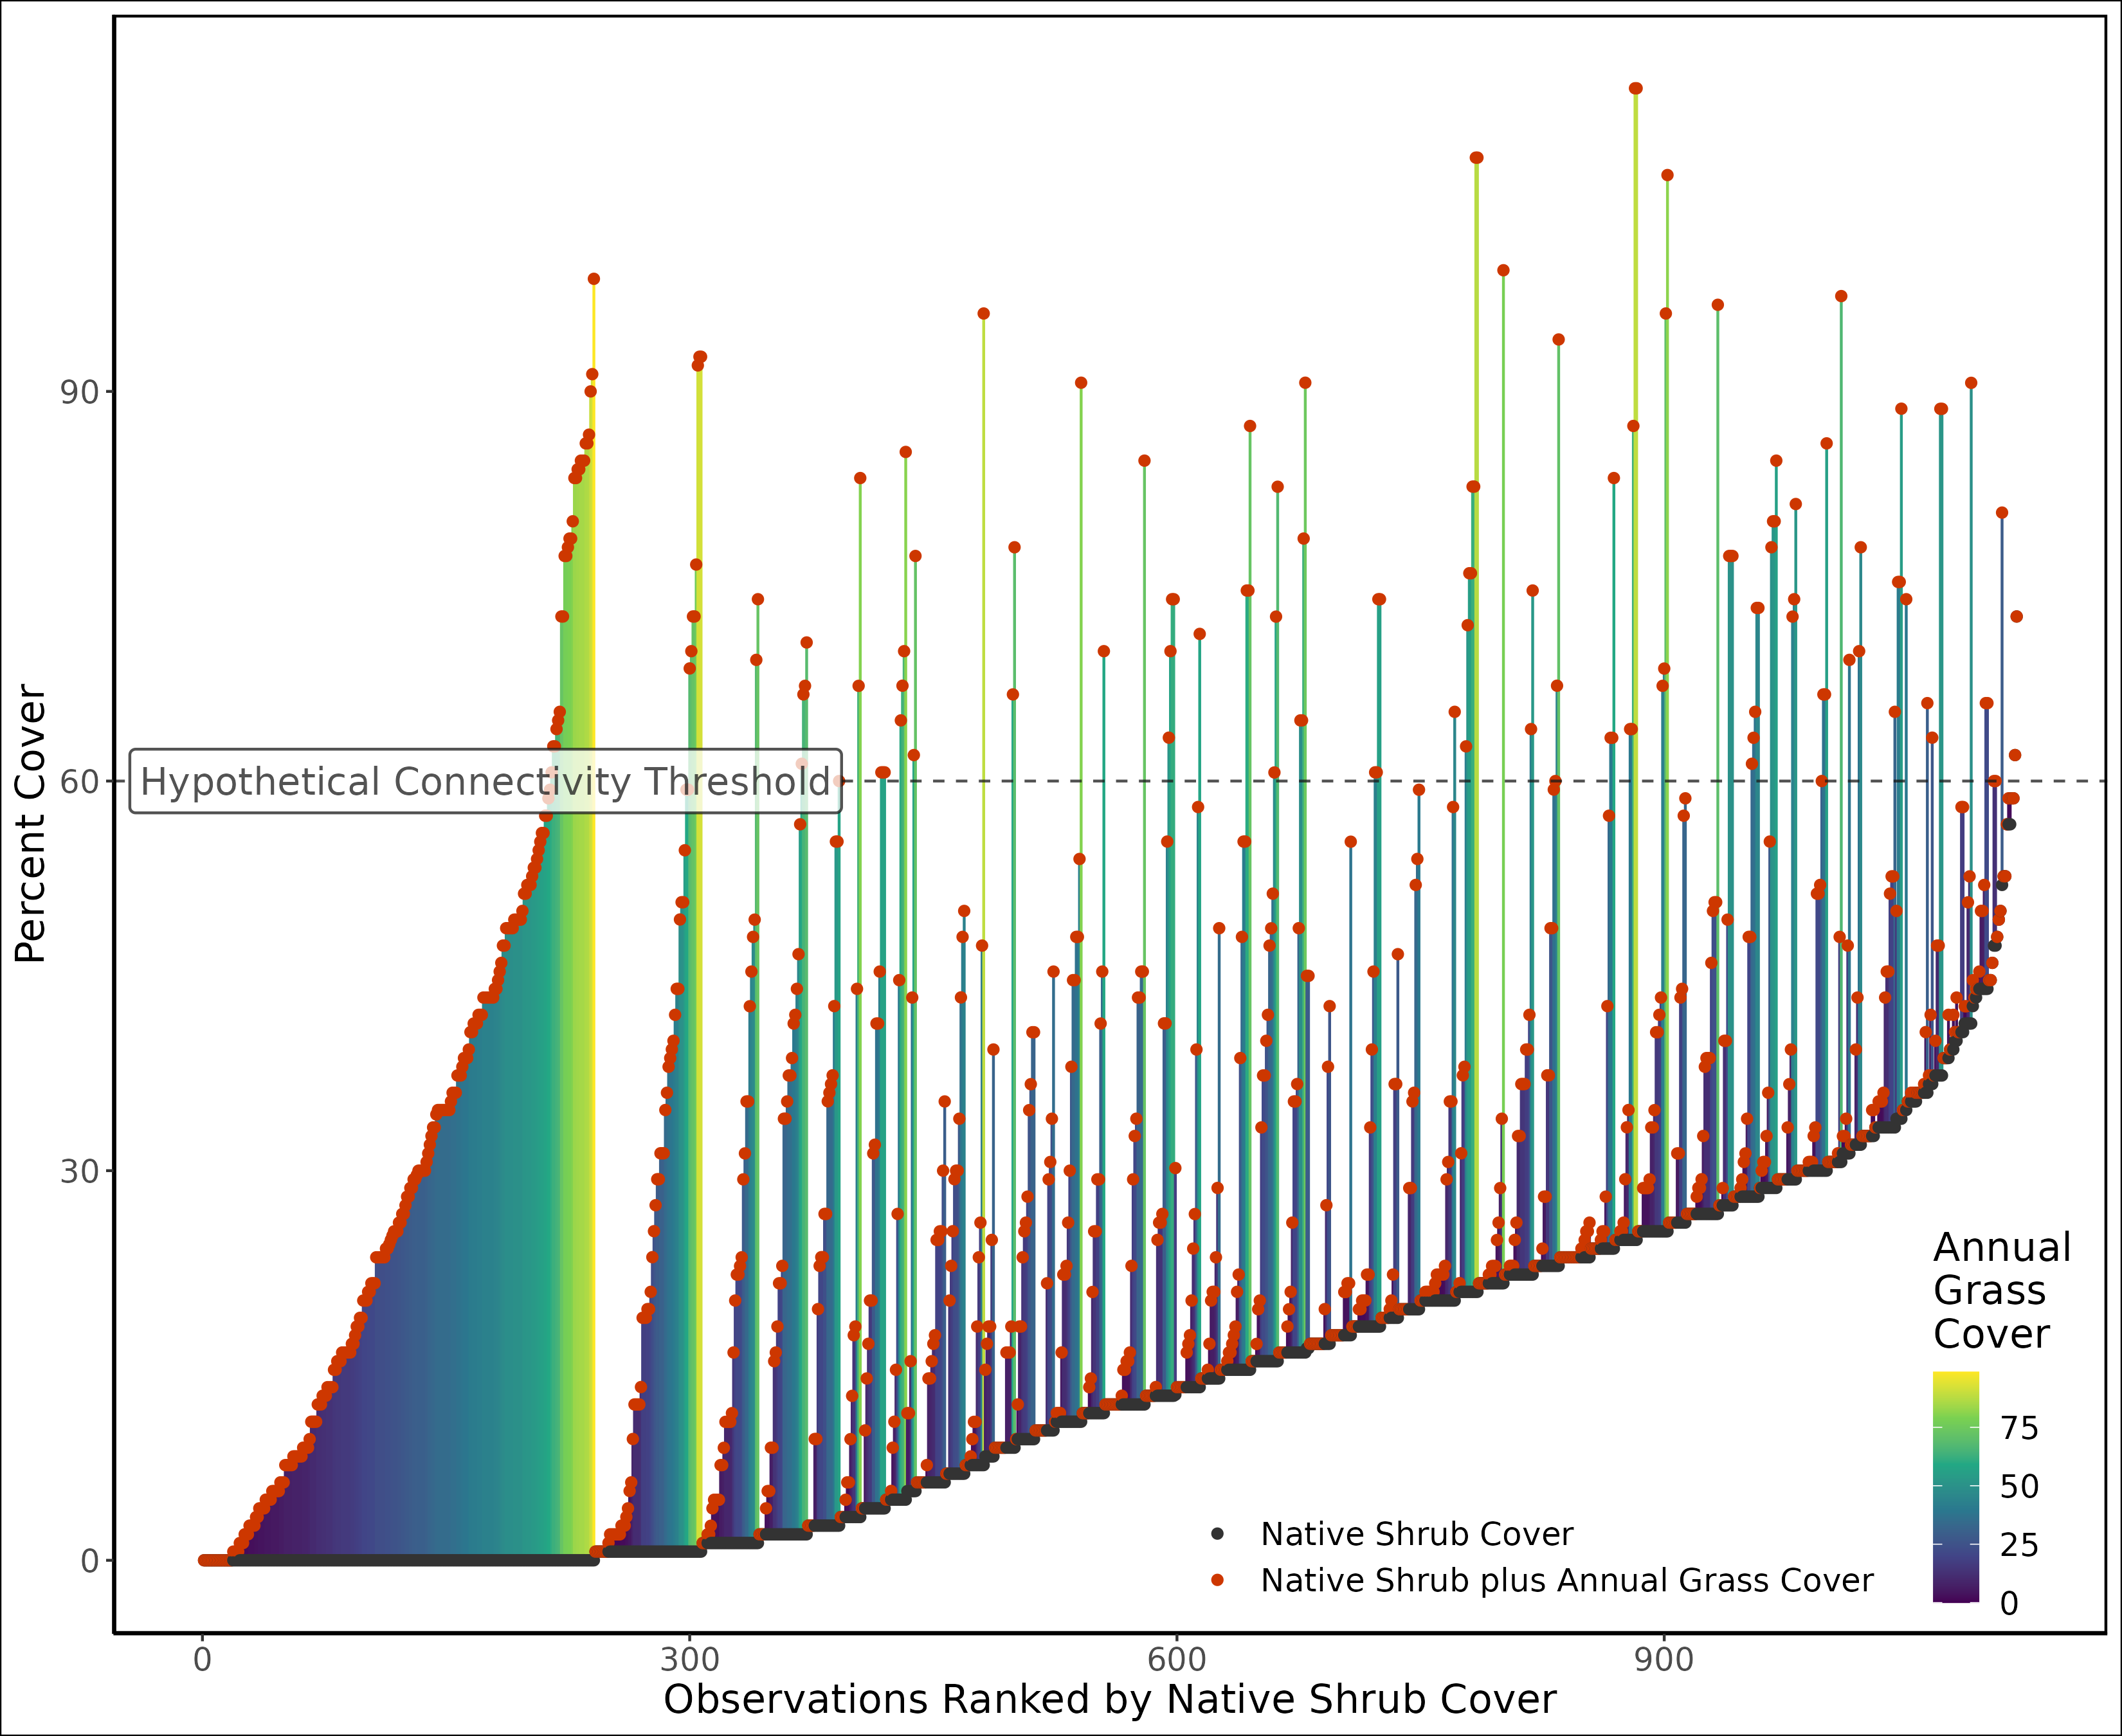
\includegraphics{images/connectivity_is_not_brte_rank_double.png}
\caption{Sites with little to no shrub cover require high IAG cover to
meet the threshold necessary to carry a fire, while sites with higher
shrub cover may reach that threshold with much lower IAG cover.
Therefore, annual grass cover alone may not be sufficient for
quantifying fire risk. Data Source: the Bureau of Land Managaement's
Assessment, Inventory and Monitoring dataset.}
\end{figure}

\newpage

\begin{figure}
\centering
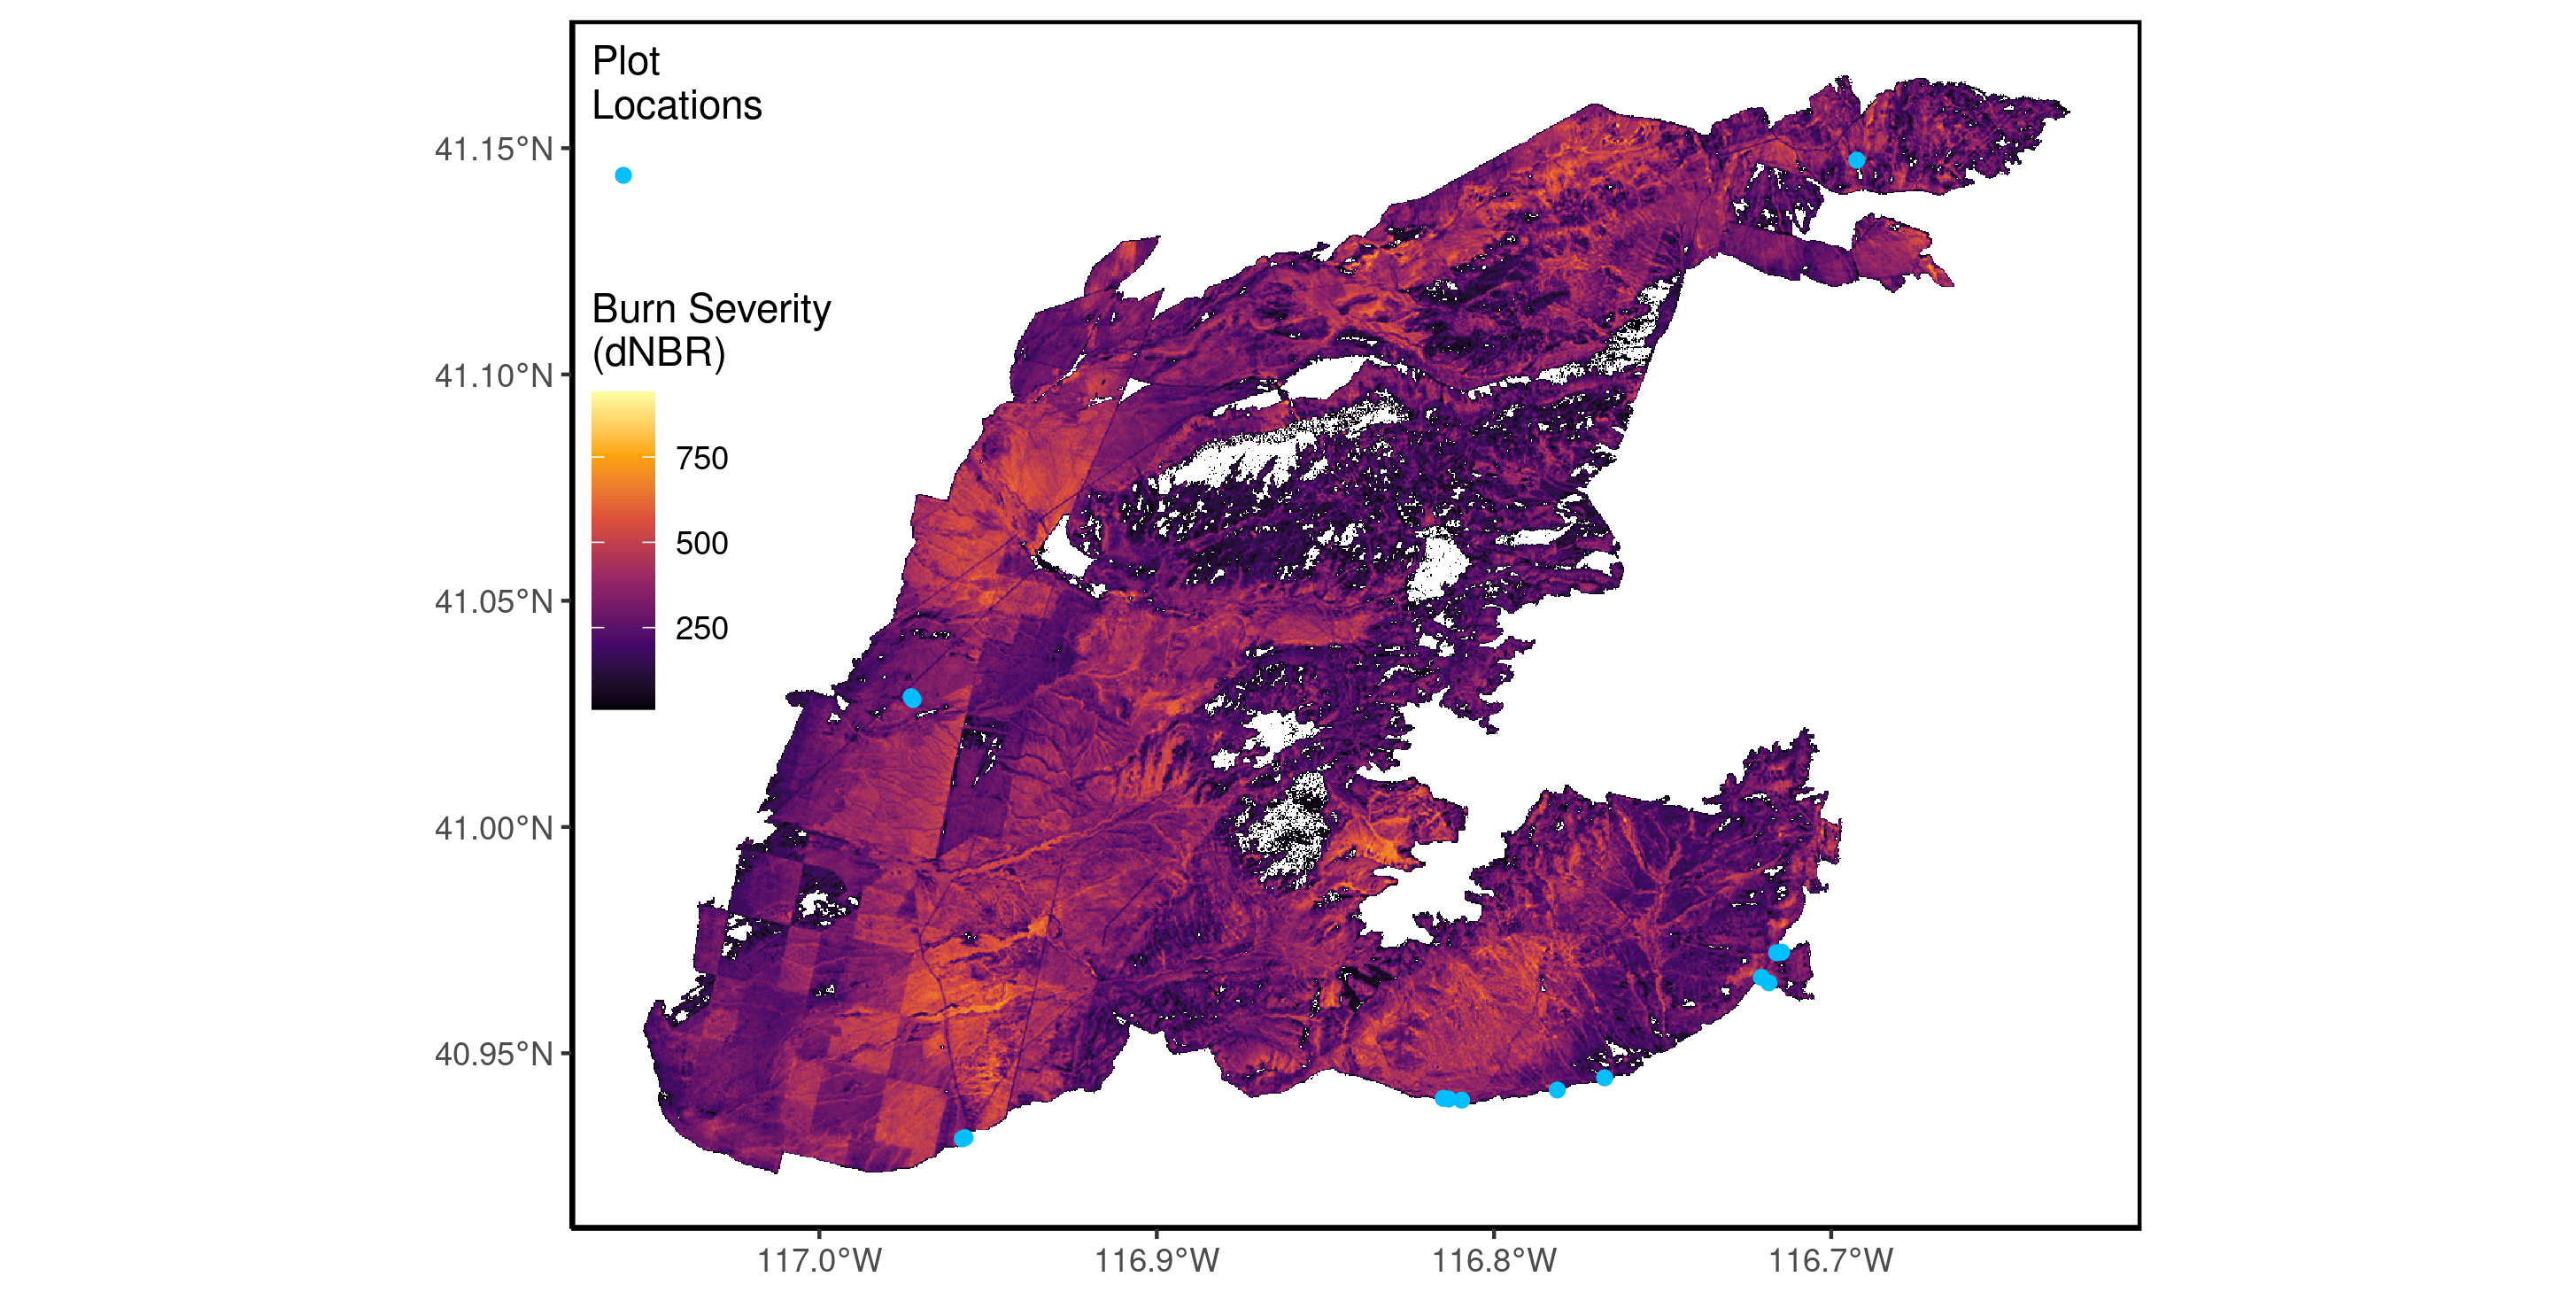
\includegraphics{images/map.png}
\caption{The 2016 Hot Pot Fire. Blue points represent sampling locations
and the shaded color is the burn severity. The checkerboard pattern on
the lower left corresponds to patterns of land ownership.}
\end{figure}

\newpage

\begin{figure}
\centering
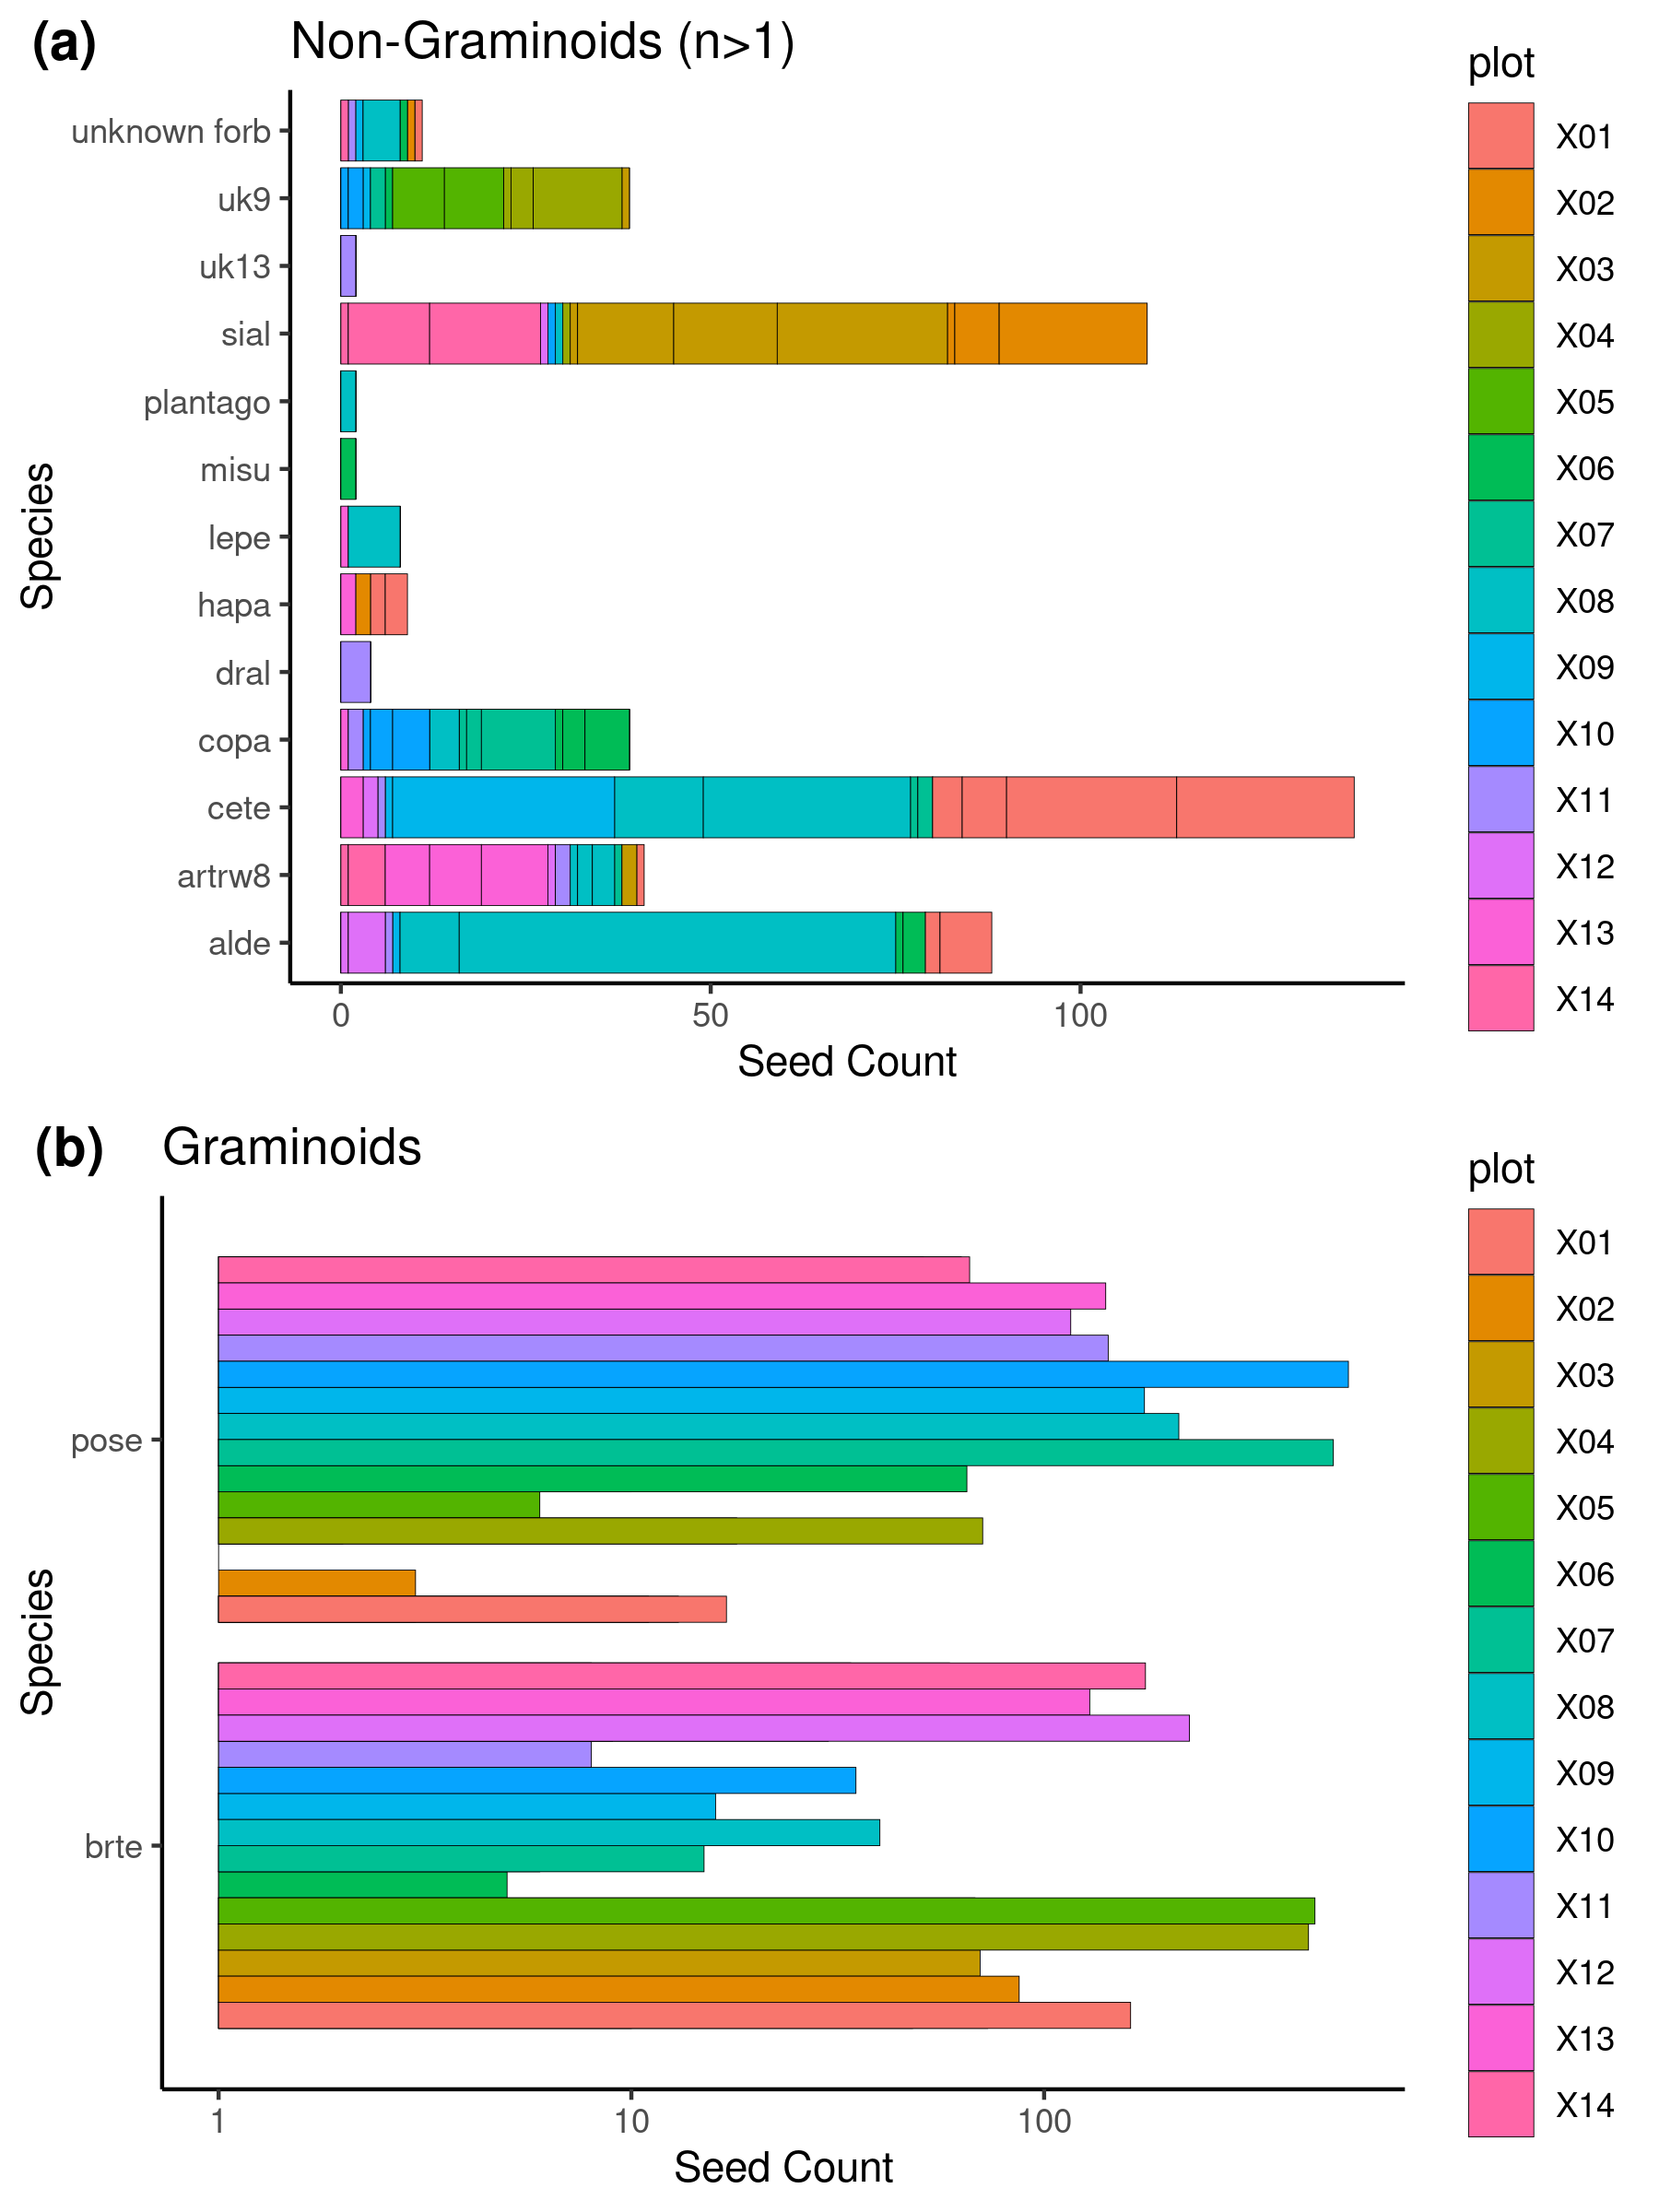
\includegraphics{images/seed_counts.png}
\caption{Seed counts by species that occurred more than once. Panel a
shows non-graminoids, b shows graminoids.}
\end{figure}

\newpage

\begin{figure}
\centering
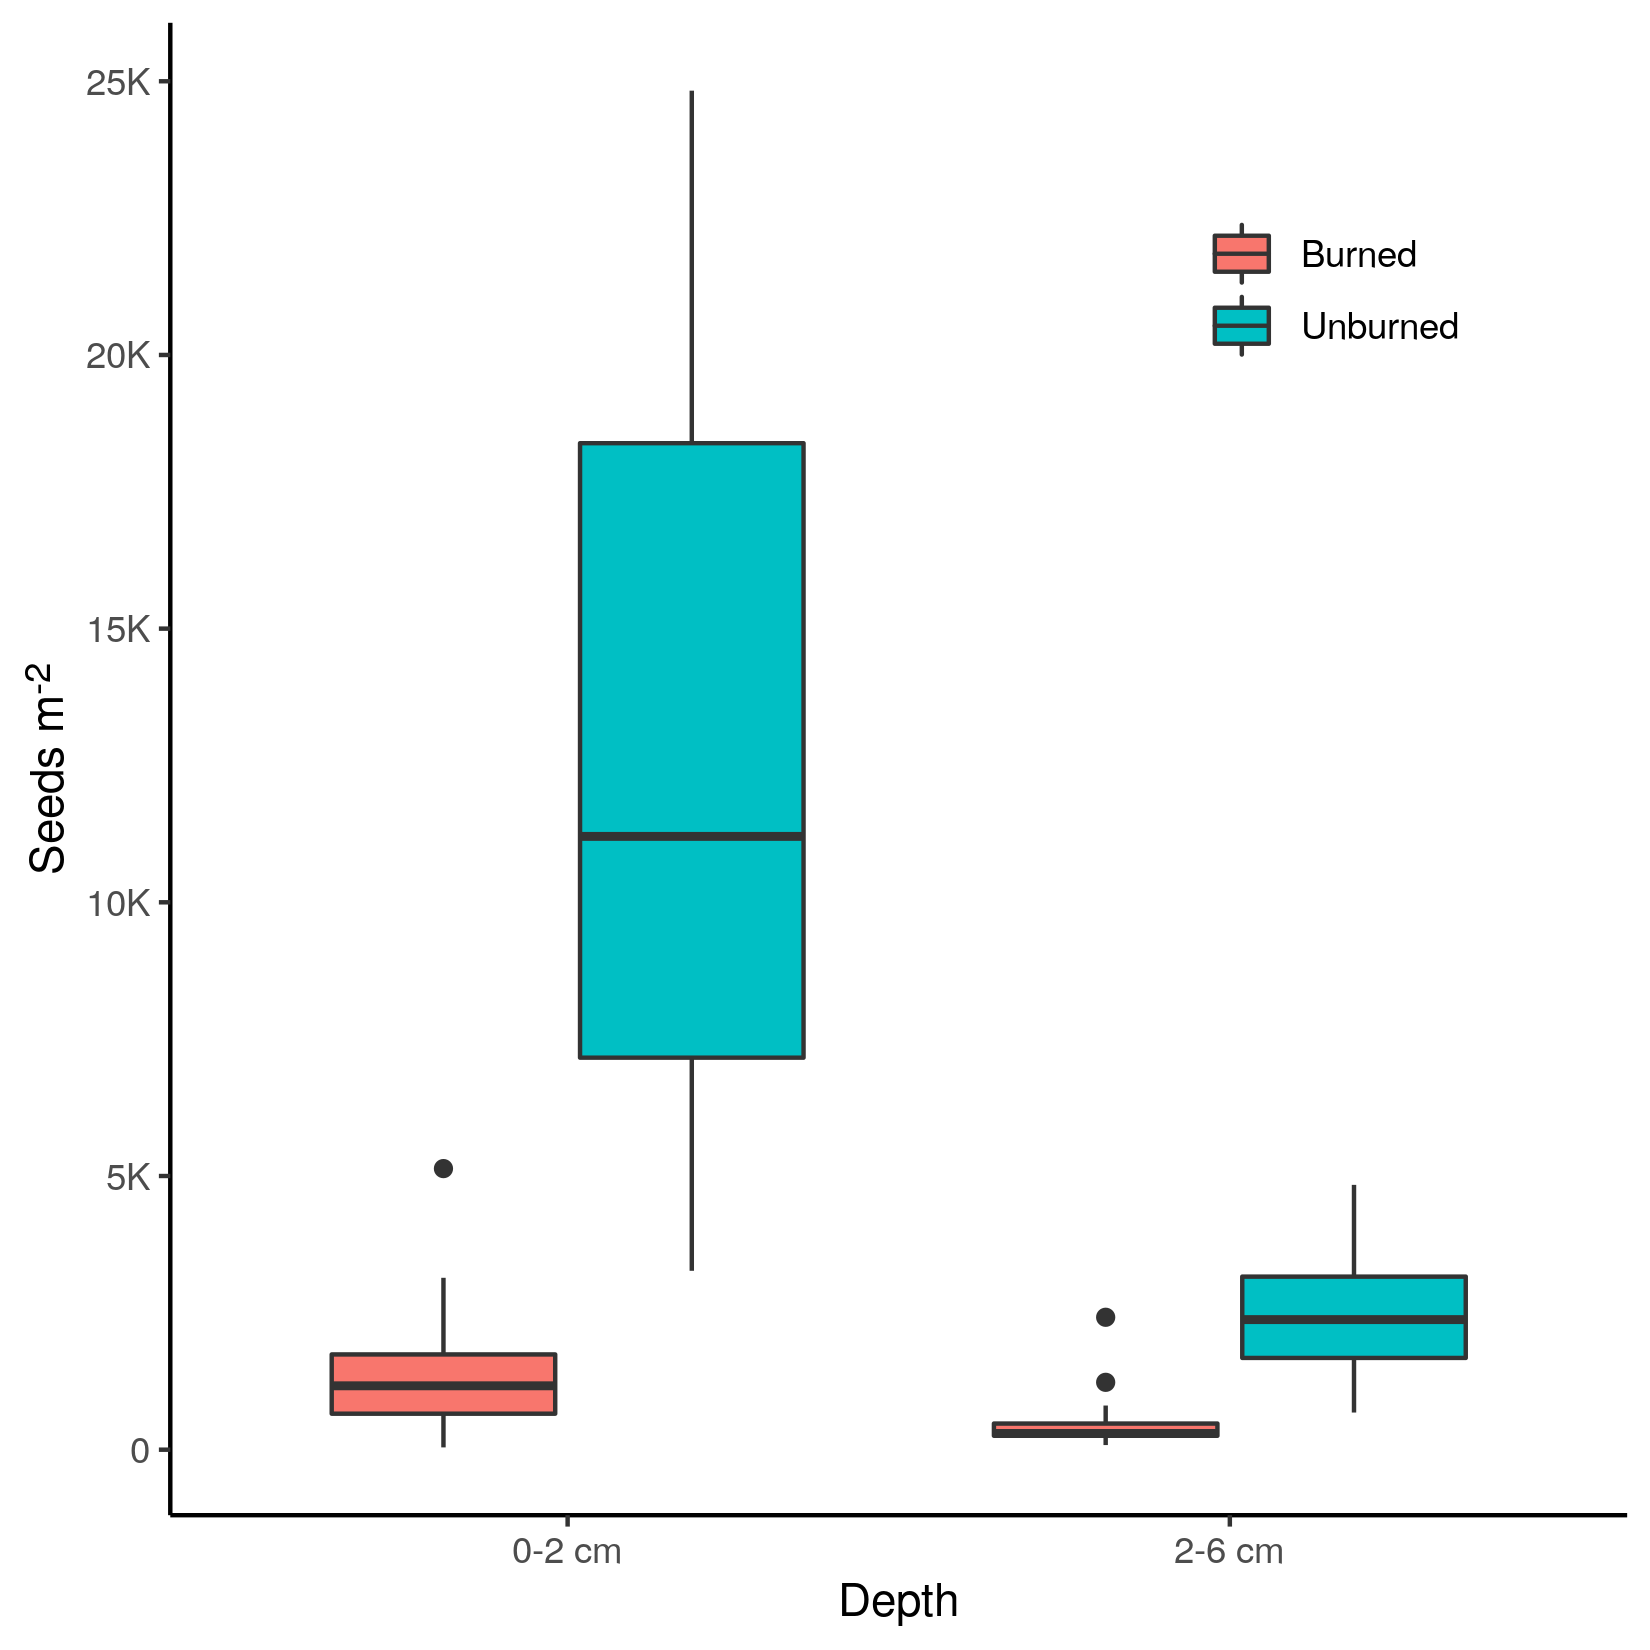
\includegraphics{images/depth_x_burned_counts.png}
\caption{Total seed counts per plot.}
\end{figure}

\newpage

\begin{figure}
\centering
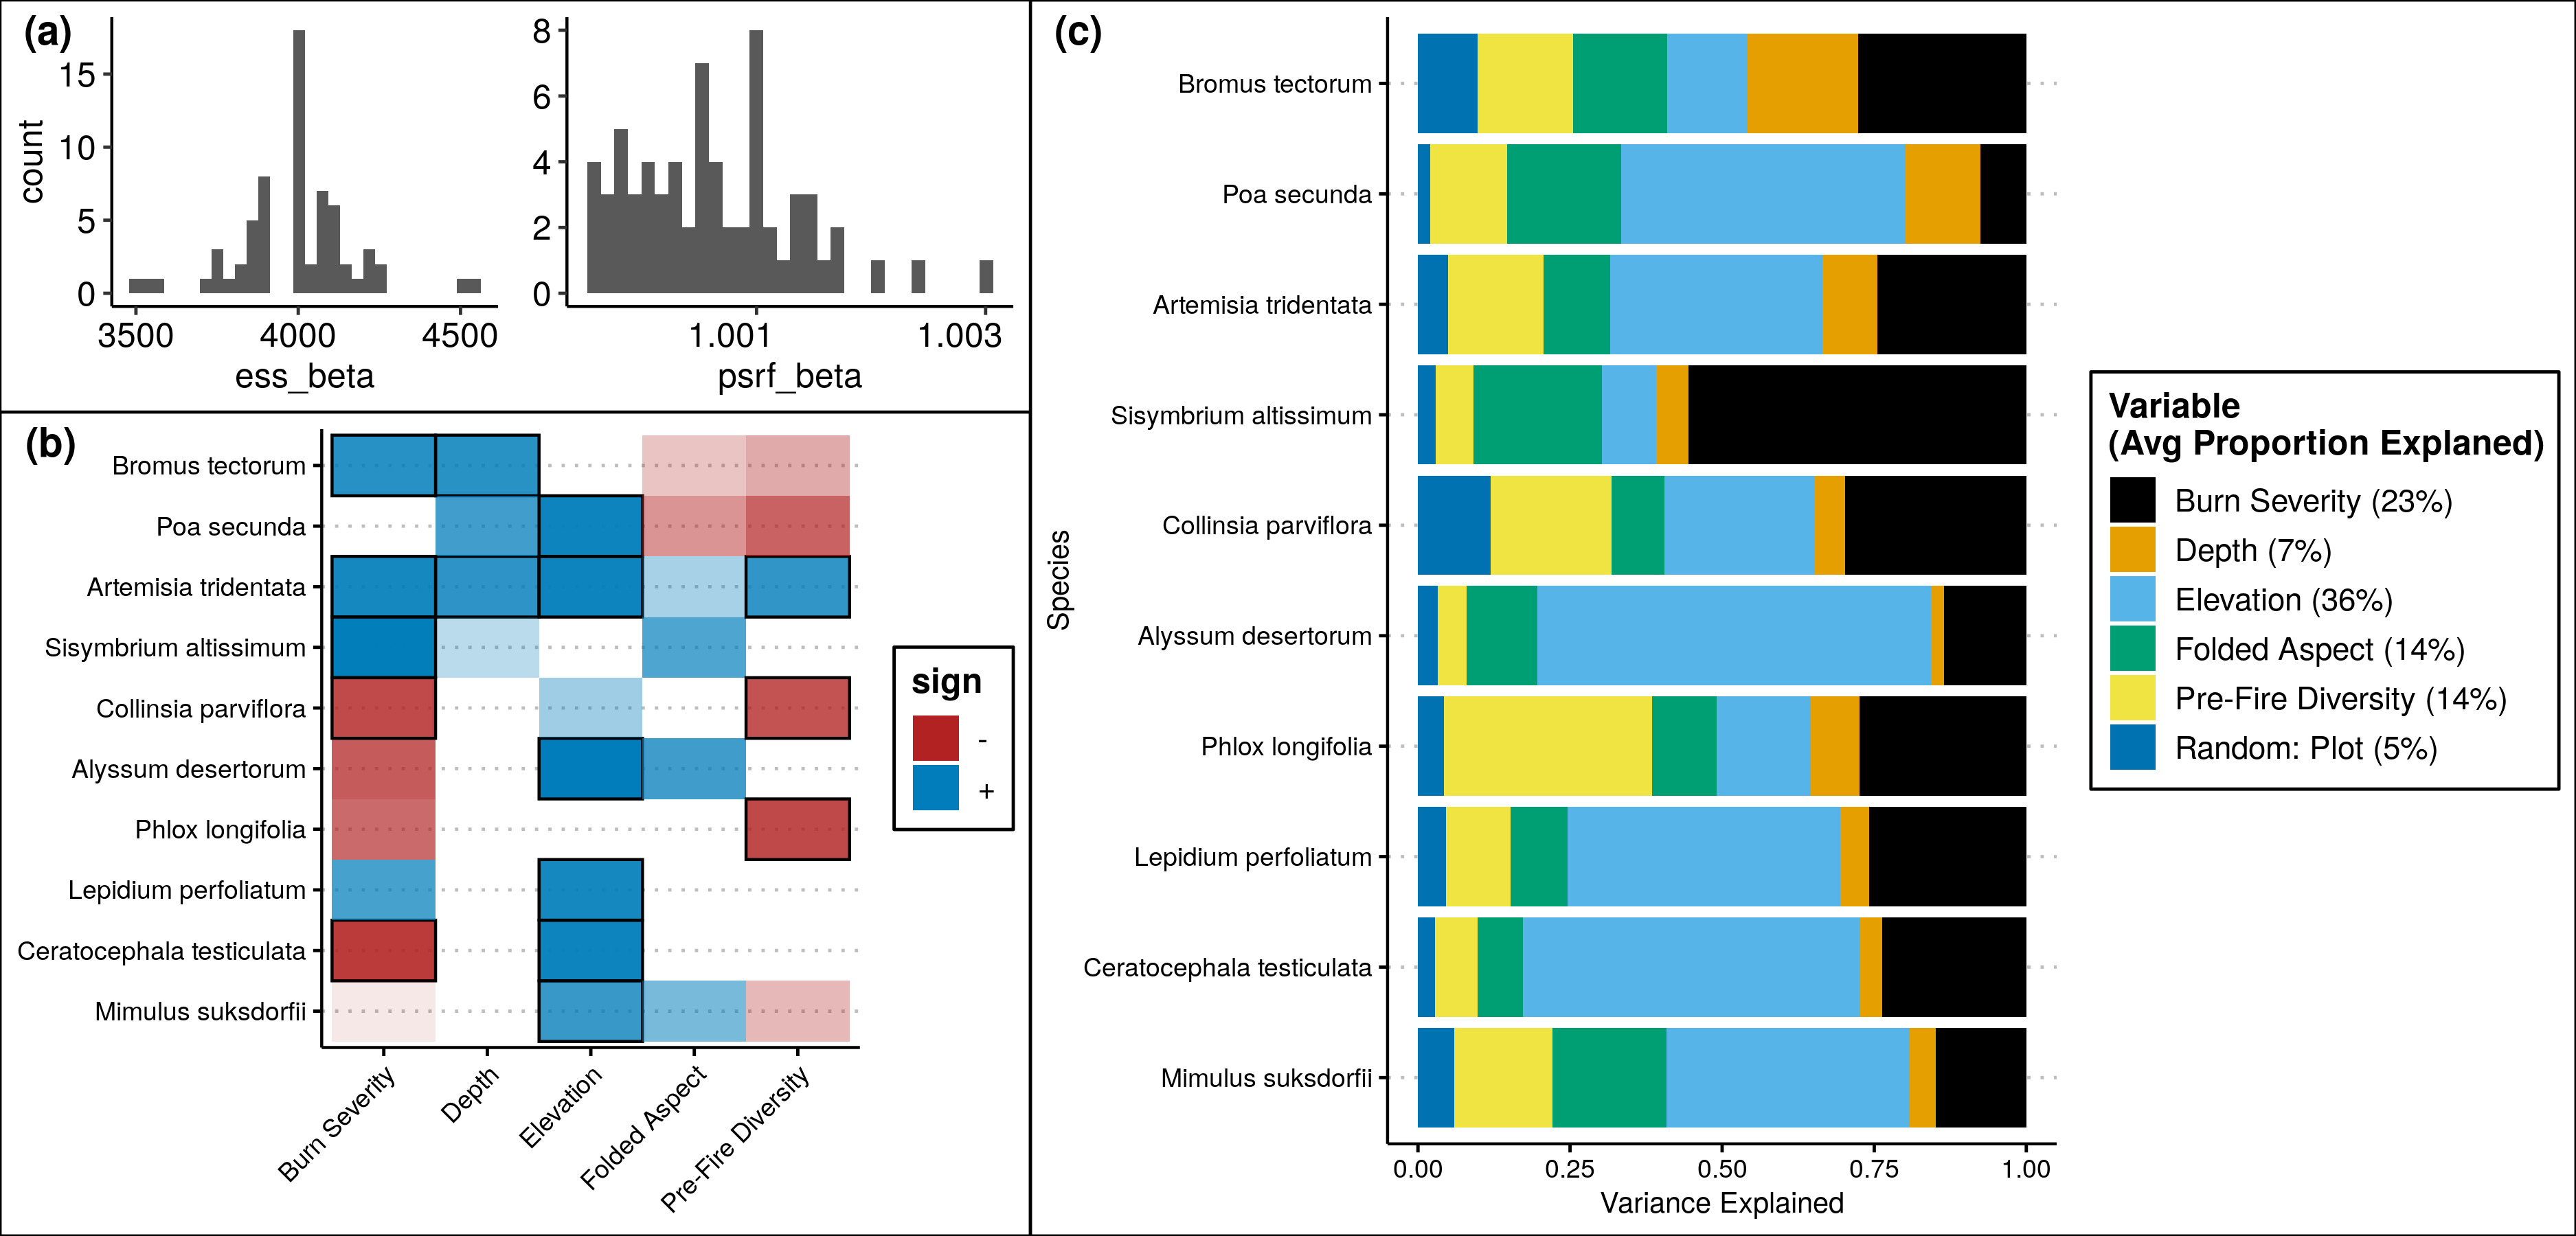
\includegraphics{images/jsdm_stuff.png}
\caption{a) Model convergence diagnostics. On the left is the effective
sample size after adjusting for autocorrelation (ideally 4,000), and on
the right is the Gelman diagnostic, ideally 1. b) Predictor variables
that had at least 80\% support. Variables with 95\% support are outlined
in black. The level of transparency corresponds to the level of support.
c) Variance partitioning by species. Average across all species per
variable is given in the legend. Species are ordered by prevalence.}
\end{figure}

\newpage

\begin{figure}
\centering
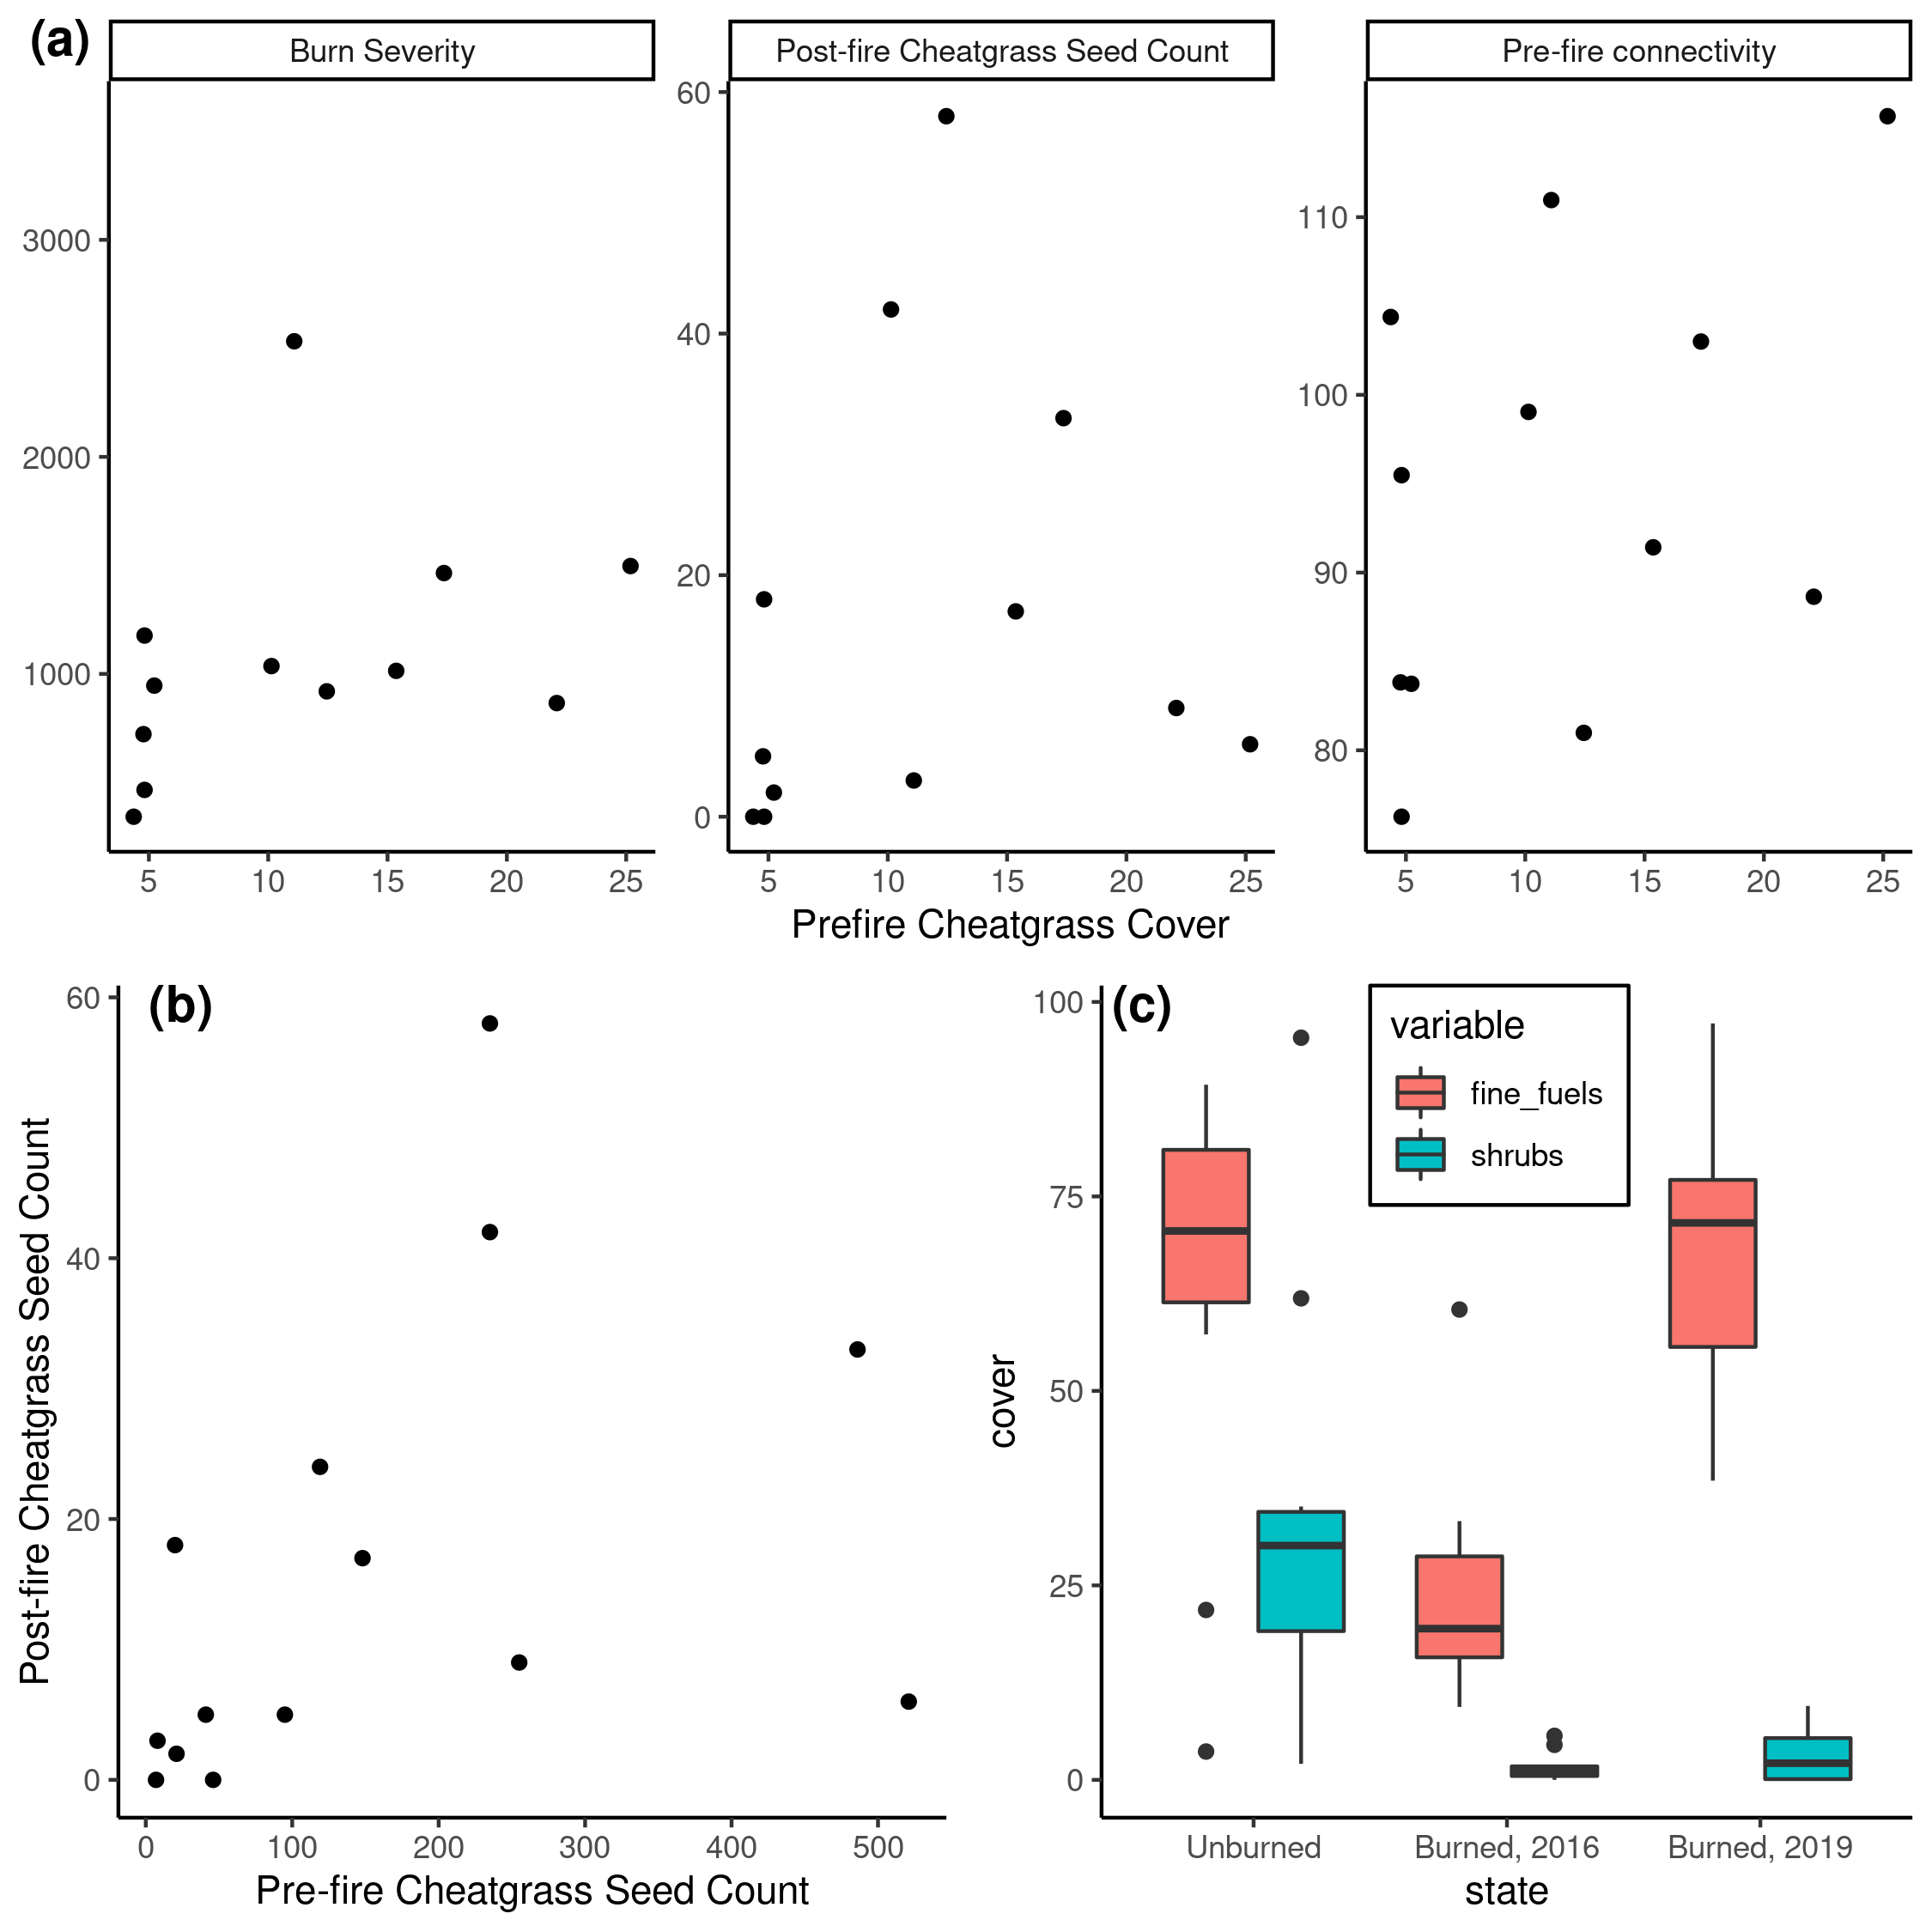
\includegraphics{images/revresp1.png}
\caption{Panel a illustrates how we did not find convincing evidence
that pre-fire cheagrass cover alone was predictive of any of the key
components of our hypothesized feedback loop. Panel b shows how even
pre-fire cheatgrass seed counts were not predictive of post-fire seed
counts. Panel c shows the general change in structural composition, from
woody to herbaceous, before and after the fire.}
\end{figure}

\newpage

\begin{figure}
\centering
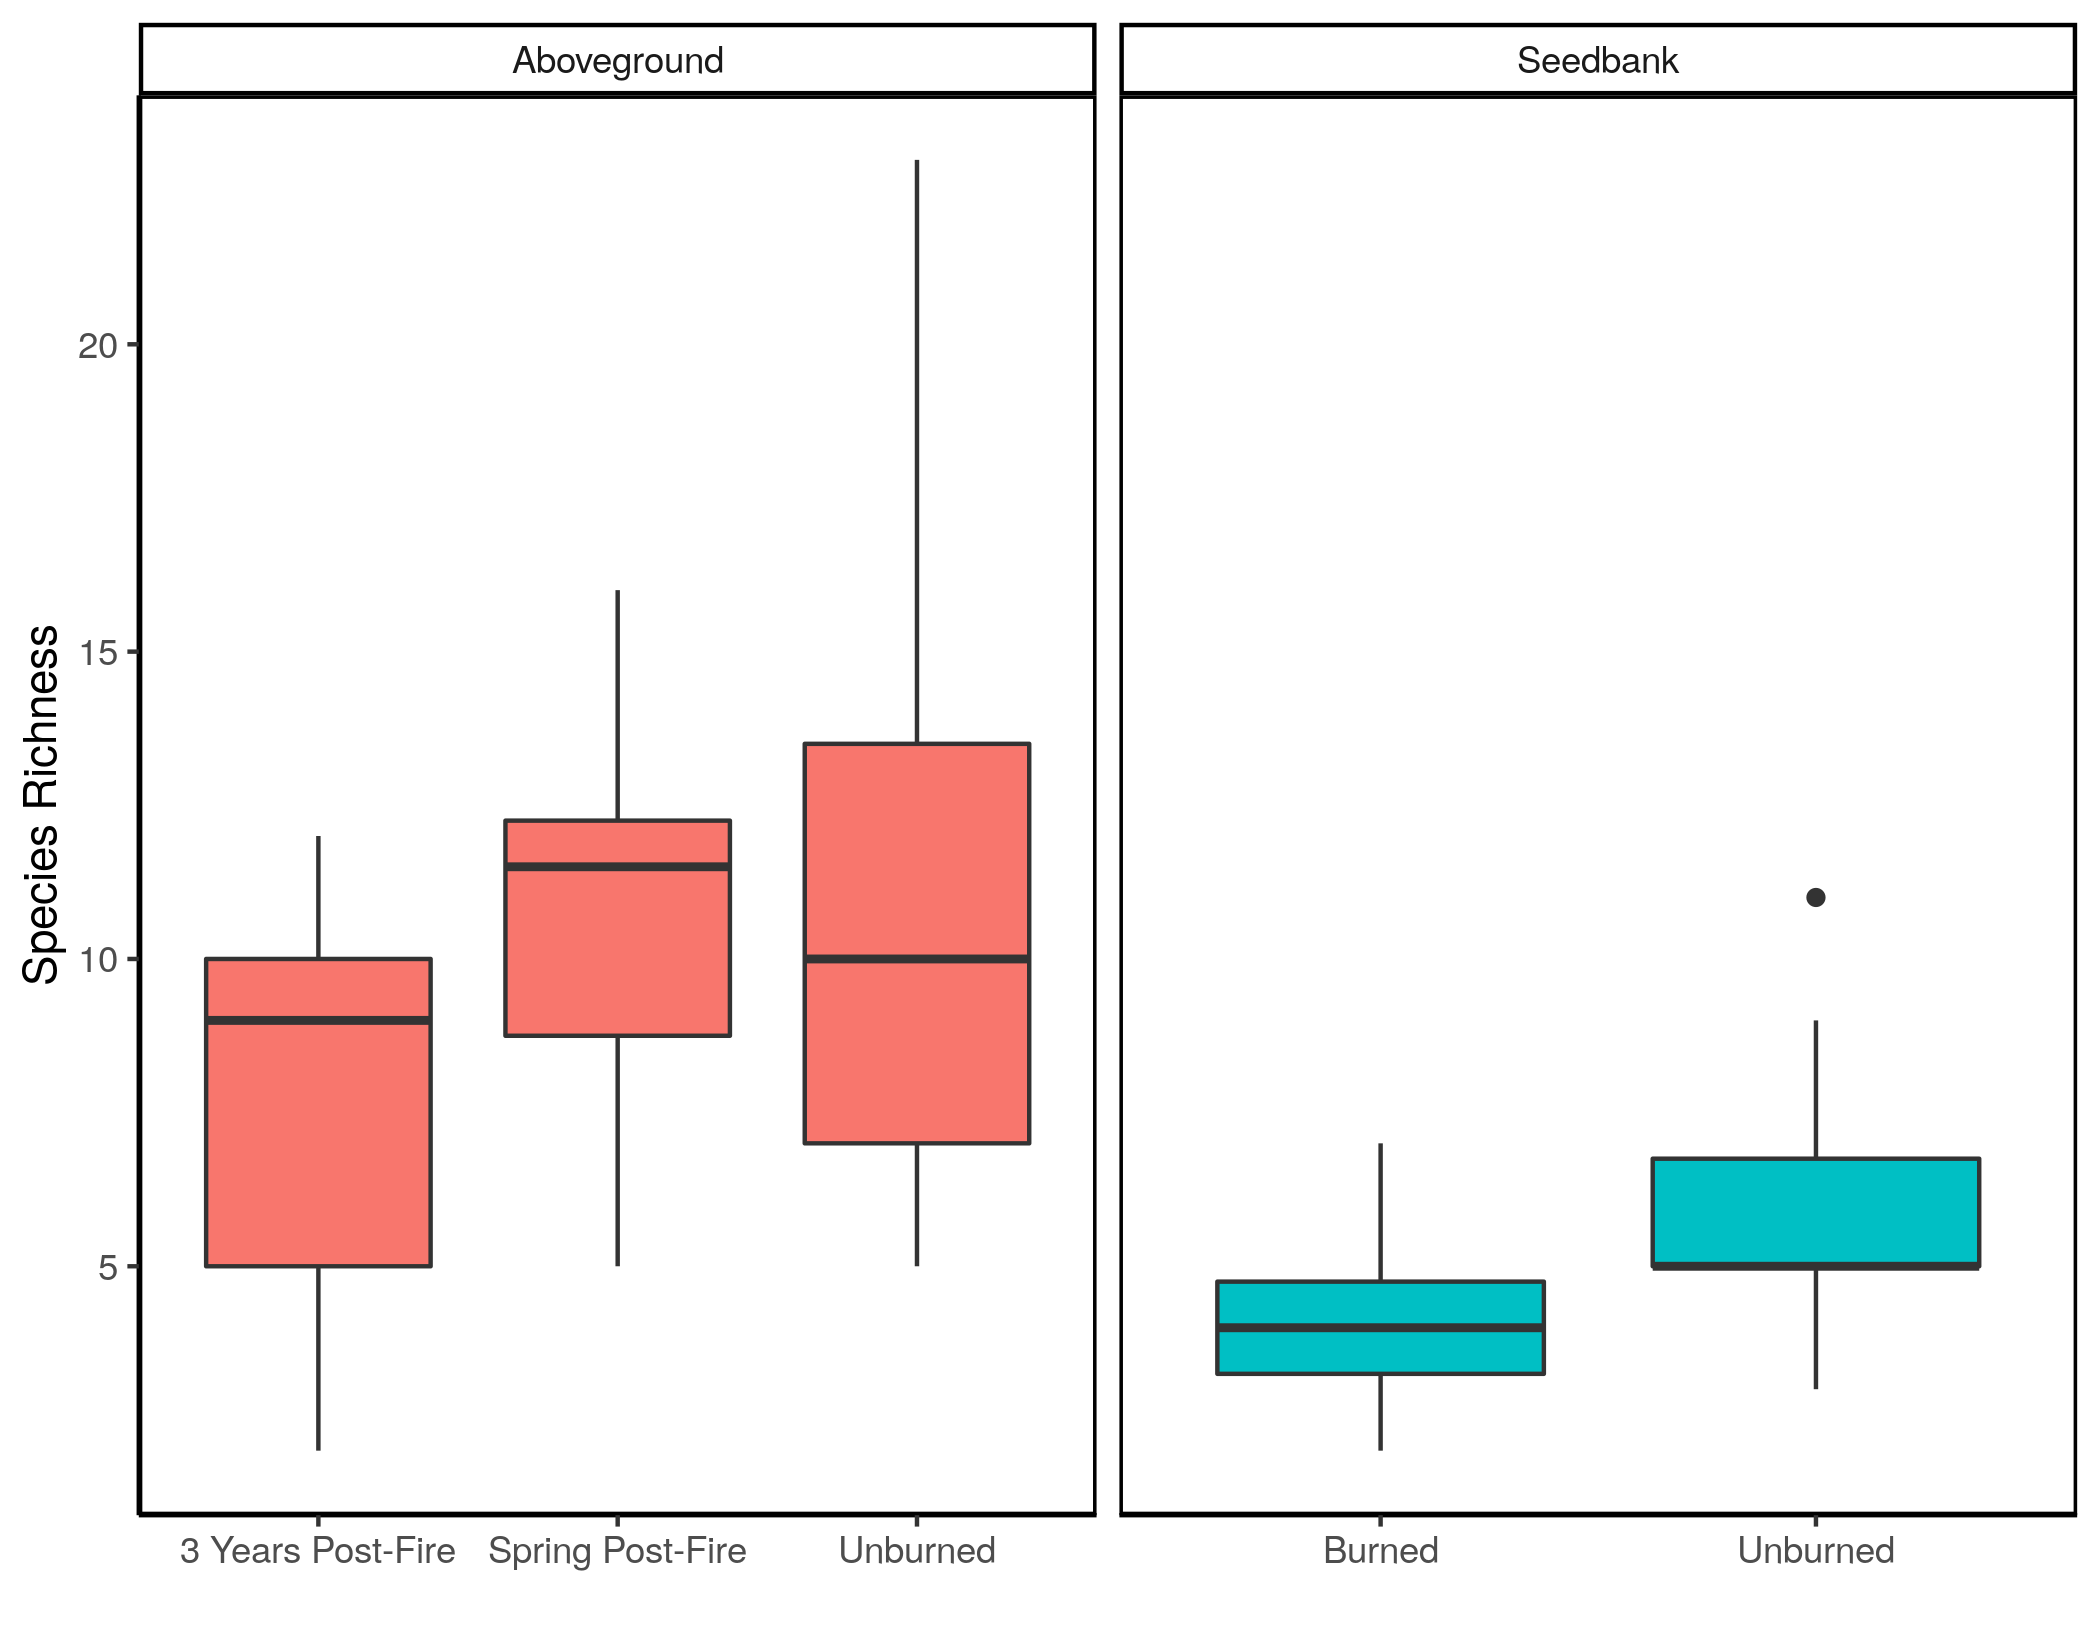
\includegraphics{images/richness_fig.png}
\caption{Species richness at different sampling times and locations.}
\end{figure}

\end{document}
